\subsection{Structure of Storage Media}\label{subsec:Structure_Storage_Media}
In this section, the structure of secondary storage is discussed.
Starting with the physical structure of magnetic disks, magnetic tapes, and solid-state storage.

\subsubsection{Magnetic Disks}\label{subsubsec:Magnetic_Disks}
Magnetic disks (typically called hard drives) provide the bulk of storage.
Inside each unit, there are disk platters that have a flat circular shape.
The two surfaces of a platter are covered with a magnetic material.
Information is stored by recording it magnetically on the platters.
Typical disks can transfer several megabytes of data per second, and they have seek times and rotational latencies of several milliseconds.

\begin{itemize}[noitemsep]
\item A read–write head ``flies'' just above each surface of every platter.
\item The heads are attached to a disk arm that moves all the heads as a unit.
\item The surface of a platter is logically divided into circular tracks, which are subdivided into sectors.
\item The set of tracks that are at one arm position makes up a cylinder.
\end{itemize}

\begin{figure}[h!tbp]
  \centering
  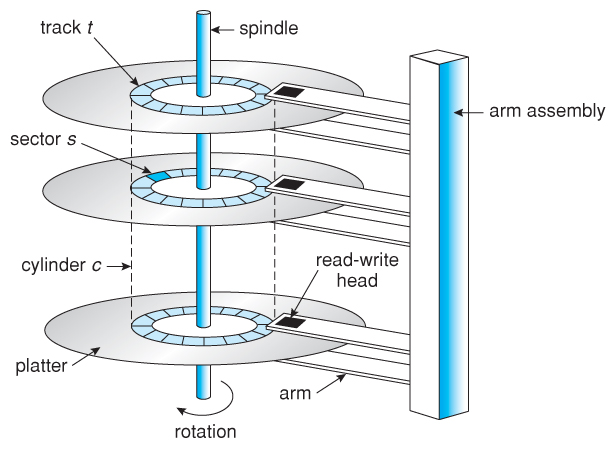
\includegraphics[scale=0.8]{./Drawings/EDAF35-Operating_Systems/Magnetic_Disk_Mechanism.jpg}
  \caption{Magnetic Disk Moving head Mechanism}
  \label{fig:HDD_Mechanism}
\end{figure}

When the disk is in use, a drive motor spins it at high speed.
Common drives spin at \SIlist{5400; 7200; 10000; 15000}{\rpm}.
Disk speed has two parts.
\begin{enumerate}[noitemsep]
\item The transfer rate is the rate at which data flow between the drive and the computer.
\item The positioning time, or random-access time. Itself consisting of 2 parts:
  \begin{enumerate}[noitemsep]
  \item Time necessary to move the disk arm to the desired cylinder, called the seek time,
  \item Time necessary for the desired sector to rotate to the disk head, called the rotational latency.
  \end{enumerate}
\end{enumerate}

There is a danger that the head will make contact with the disk surface.
This accident is called a head crash, and cannot be repaired; the entire disk must be replaced.

A disk drive is attached to a computer by an I/O bus.
Several kinds of buses are available, including:
\begin{itemize}[noitemsep]
\item Advanced Technology Attachment (ATA)
\item Serial ATA (SATA)
\item eSATA
\item Universal Serial Bus (USB)
\item Fiber Channel (FC)
\end{itemize}

The data transfers on a bus are carried out by special electronic processors called controllers.
\begin{description}[noitemsep]
\item[Host Controller:] The controller at the computer end of the bus.
\item[Disk Controller:] Built into each disk drive.
\end{description}

To perform a disk I/O operation, the computer places a command into the host controller, typically using memory-mapped I/O ports.
The host controller then sends the command via messages to the disk controller, and the disk controller operates the disk-drive hardware to carry out the command.

\subsubsection{Magnetic Tapes}\label{subsubsec:Magnetic_Tapes}
Magnetic tapes are relatively permanent and can hold large quantities of data, its access time is slow compared with that of main memory and magnetic disk.
In addition, random access to magnetic tape is about a thousand times slower than random access to magnetic disk, so tapes are not very useful for active secondary storage.

A tape is kept in a spool and is wound or rewound past a read–write head.
Moving to the correct spot on a tape can take minutes, but once positioned, tape drives can write data at speeds comparable to disk drives.
Tape capacities vary greatly, depending on the particular kind of tape drive


%%% Local Variables:
%%% mode: latex
%%% TeX-master: "../../EDAF35-Operating_Systems-Reference_Sheet"
%%% End:
